\section{Model architecture}
\label{sec:model_architecture}

To approach the problem of error estimation, two different model architectures are devised. The first model architecture, FESDModelv1, is a deep convolutional neural network that uses the RGB, Depth, and Pose data as separate inputs. This model can be seen in figure \ref{fig:model_architecture_v1}.

\begin{figure}[ht]
  \centering
  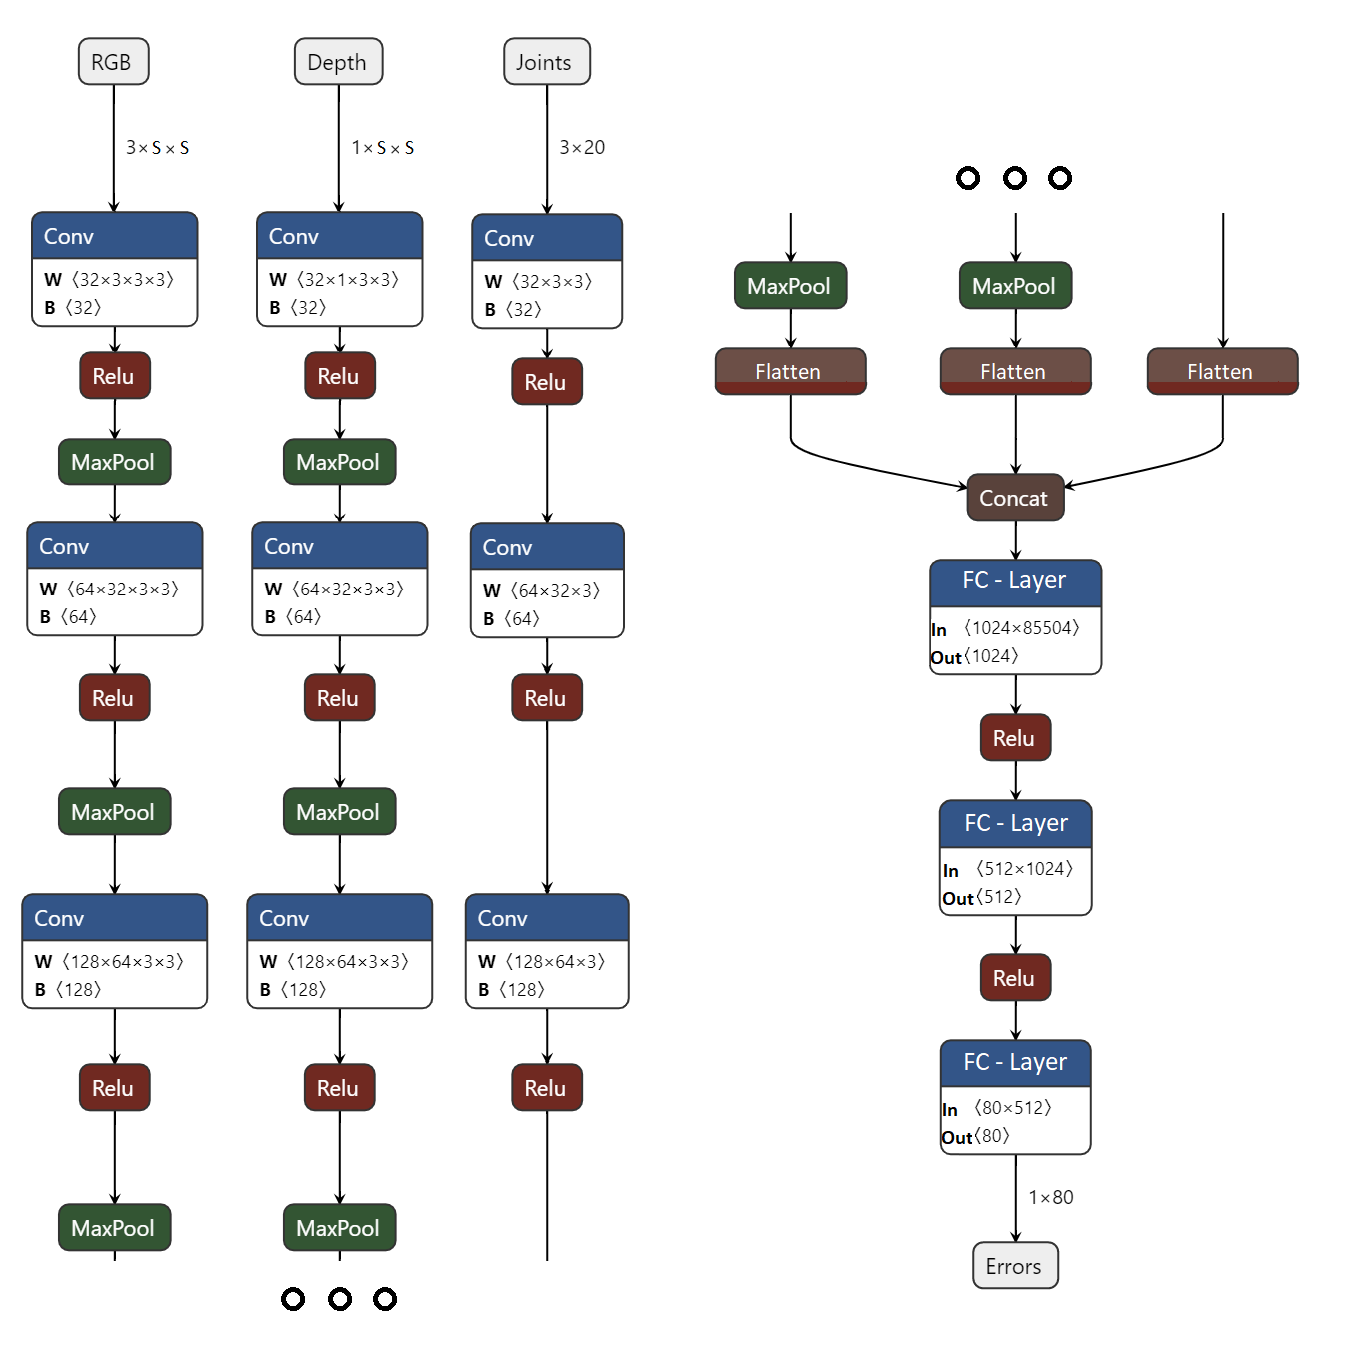
\includegraphics[width=.8\linewidth]{figures/Model/FESD.png}
  \caption[FESDModel architecture version 1]{Original FESDModel architecture with three different inputs; RGB, Depth and Joint data. With 'S' as the image size. After three convolutions the three streams are concatenated to be passed into three fully connected layers with ReLU activation functions. In this example network, the model calculates the joint problem set, therefore the output is a 1D 80 tensor of multi-object, one for each joint, i.e. 20, multi-class, one for each error class, i.e. 4, values.}
  \label{fig:model_architecture_v1}
\end{figure}

The second model architecture, FESDModelv2, utilises transfer learning to extract the features of the input data using a pre-trained model. FESDModelv2 can be seen in figure \ref{fig:model_architecture_v2}. Both models are trained to predict the error labels for each joint. The error labels are the same as the error labels used in the data labelling explained in section \ref{sec:data_labeling}. The fully connected layers of both networks use intermittent rectified linear unit (ReLU) activation functions to combat the vanishing gradient problem by passing only the values which are greater than zero into the next layer.

\begin{figure}[ht]
  \centering
  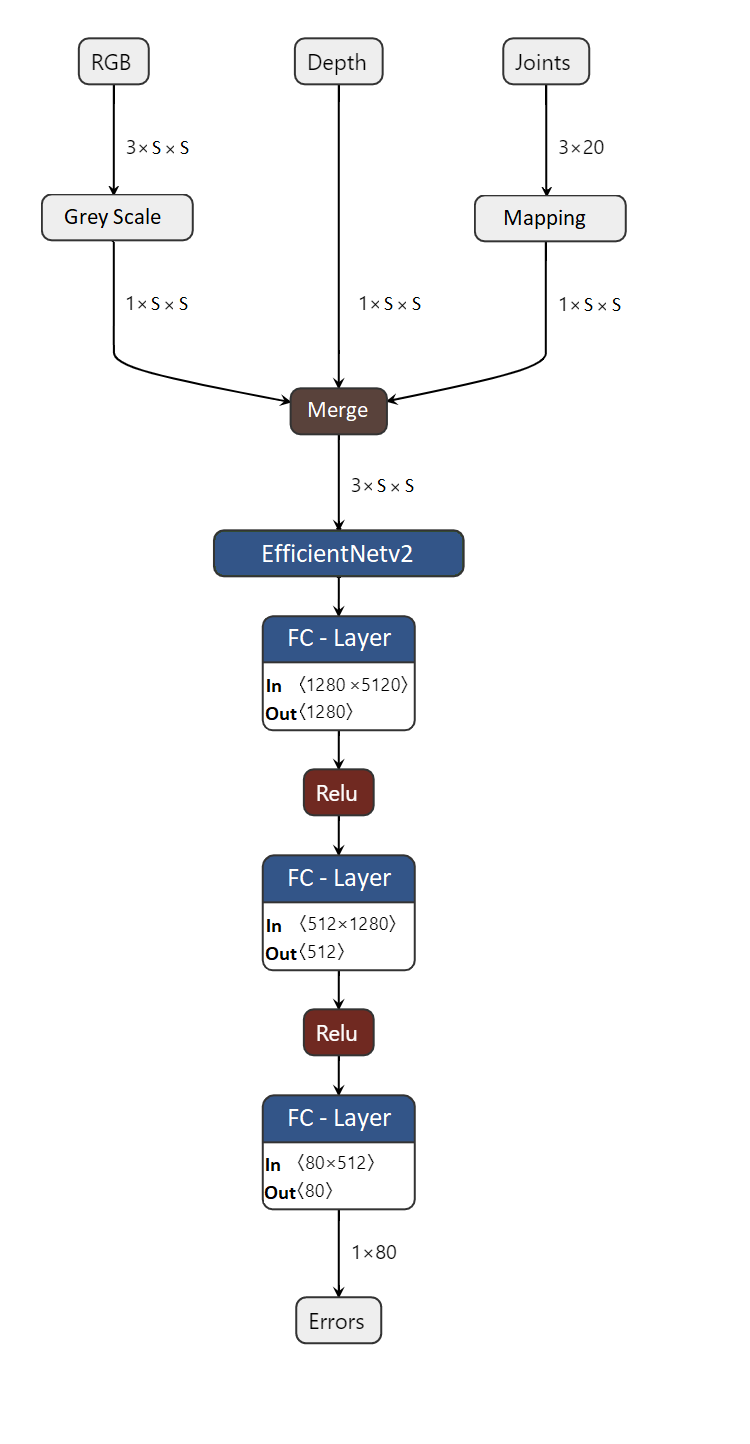
\includegraphics[width=.5\linewidth]{figures/Model/FESDv2.png}
  \caption[FESDModel architecture version 2]{FESDModelv2 architecture with transfer learning. The input is merged into a single RGB image and passed into a feature extractor. With 'S' as the image size. The feature extractor is a pre-trained EfficientNet v2 S. The output of the feature extractor is passed into two fully connected layers with ReLU activation functions. In this example network, the model calculates the joint problem set, therefore the output is a 1D 80 tensor of multi-object, one for each joint, i.e. 20, multi-class, one for each of the 4 error classes.}
  \label{fig:model_architecture_v2}
\end{figure}

While FESDModelv1 uses the data as it is stored in the dataset, FESDModelv2 merges the data into a single RGB image. This is done using the feature extractor, which is trained on RGB images. The data is merged by assigning each modality to a channel in an RGB image. The RGB image is transformed into greyscale and assigned to the red channel, the depth image is scaled to a value between 0 and 255 and assigned to the green channel, and the joint coordinates are assigned to the blue channel.

In total eight models were developed and trained. Four models were trained using FESDModelv1 and four models were trained using FESDModelv2. Each of the models corresponds to one of the problem sets introduced in section \ref{sec:problem_set}, i.e. one model for each problem set is trained using FESDModelv1 and one model for each problem set is trained using FESDModelv2.

The output of the model varies depending on the problem set. The joint problem set contains more detailed error information, which was discussed in section \ref{sec:data_labeling}. Therefore, the models developed to detect joint-level errors have an output vector of size 80, i.e. twenty joints, each with four different error labels. The other problem sets are labelled using two values to represent whether an area is faulty, "Error" or "No Error". Hence the Full Body, Half Body and Body Part problem sets have an output vector of size 2, 4, and 12 respectively.

To choose a network that is used by FESDModelv2 as a feature extractor, multiple different networks have been compared, which can be seen in figure \ref{fig:network_comparison}. One of the target applications of the model is to be used in a real-time application so that error handling can be conducted. Consequently, a lightweight model which does not impact the performance much is preferred. Therefore, the models are compared by the number of floating-point operations (FLOPS) to their Accuracy on ImageNet-1K. Table \ref{tab:network_comparison} shows the top 5 models according to their accuracy and performance. 

\begin{figure}[ht]
  \centering
  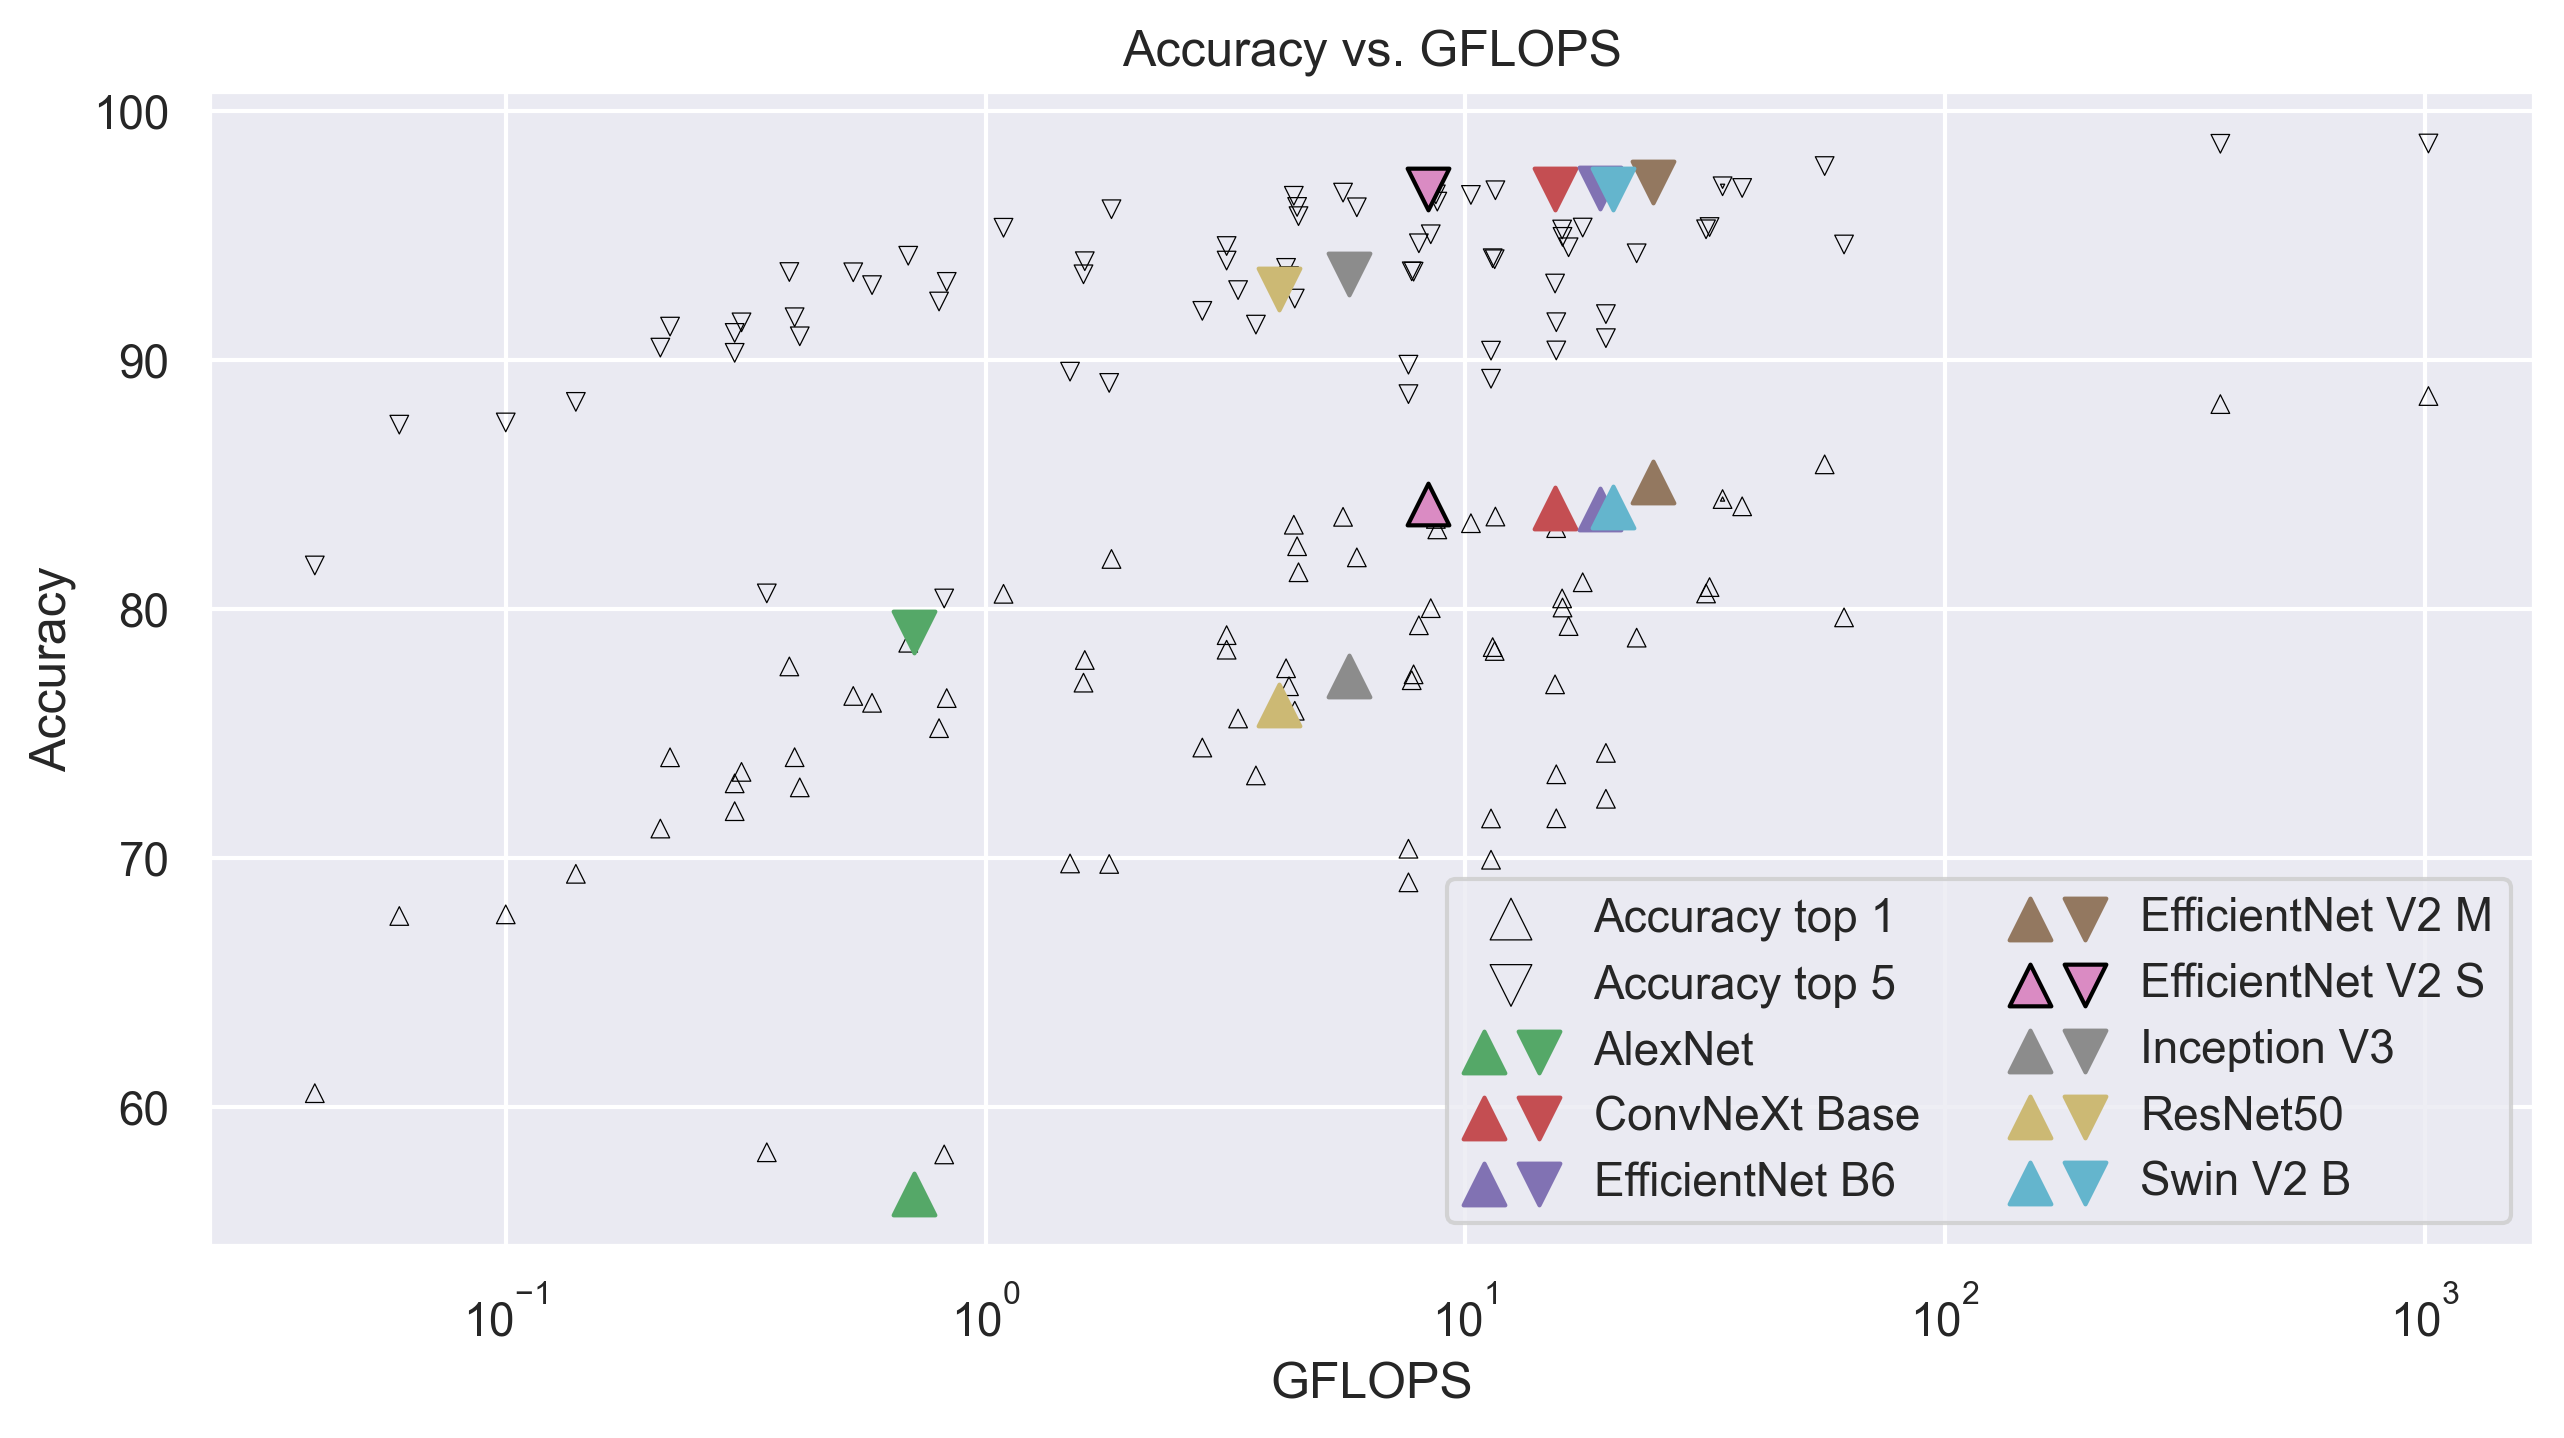
\includegraphics[width=.8\linewidth]{figures/network/networks.png}
  \caption[Network comparison]{The comparison of different networks by their GFLOPS and their Top-5 Accuracy. The models are sorted by their GFLOPS and their Top-5 Accuracy\footnote{Source: \url{https://pytorch.org/vision/main/models.html} on 08/05/2023}. The models are EfficientNet V2 S, ConvNeXt Base, EfficientNet B6, Swin V2 B, and EfficientNet V2 M. Additionally, AdamNet, ResNet-50 and Inception-v3 are added as a reference.}
  \label{fig:network_comparison}
\end{figure}

\begin{table}[ht]
  \caption[Top 5 models for Accuracy and Performance]{The top 5 models according to their accuracy and performance. The models are sorted by their GFLOPS and their Top-5 Accuracy\footnote{Source: \url{https://pytorch.org/vision/main/models.html} on 08/05/2023}. The models are EfficientNet V2 S, ConvNeXt Base, EfficientNet B6, Swin V2 B, and EfficientNet V2 M.}
  \label{tab:network_comparison}
  \centering
  \begin{tabular}{lrrrr}
    \hline
            Weight &  Acc@1 &  Acc@5 &   Params &  GFLOPs \\
    \hline
  EfficientNet V2 S & 84.228 & 96.878 & $2.15 \times 10^7$ &   8.370 \\
      ConvNeXt Base & 84.062 & 96.870 & $8.86 \times 10^7$ &  15.360 \\
    EfficientNet B6 & 84.008 & 96.916 & $4.30 \times 10^7$ &  19.070 \\
          Swin V2 B & 84.112 & 96.864 & $8.79 \times 10^7$ &  20.320 \\
  EfficientNet V2 M & 85.112 & 97.156 & $5.41 \times 10^7$ &  24.580 \\
  \hline
  \end{tabular}
\end{table}

EfficientNet v2 was chosen since it proved to be the most performant while being the most accurate of the networks that were analysed. In particular, the small variant with $2.15 \times 10^7$ Parameters and a Top-1 Accuracy of $84.228\%$\cite{tan2021efficientnetv2}.  While EfficientNet V2 M out-performs EfficientNet V2 S in terms of Top-1 Accuracy, the number of additional parameters needed to achieve a better accuracy outway the performance bonus that EfficientNetv2 S brings with it. EfficientNetv2 is a convolutional neural network, which optimises training speed and parameter efficiency and improves upon EfficientNet\cite{tan2020efficientnet}. The main focus of EfficientNet is the scaling of the model in width, depth and resolution of the input image. 
